\documentclass[10pt, aspectratio=169]{beamer}

%\usepackage[top = 1 in, bottom = 1 in, left = 1 in, right = 1 in]{geometry}

\usepackage{amsmath}
\allowdisplaybreaks[1]
\usepackage{amssymb, amsfonts}
\usepackage{enumerate}
\usepackage{multirow}
\usepackage{hhline}
\usepackage{array}
\usepackage{longtable}
\usepackage{graphicx}
\usepackage{tabularray}
\usepackage{undertilde}
\usepackage{dingbat}
\usepackage{fontawesome5}
\usepackage{tasks}
\usepackage{bbding}
\usepackage{twemojis}
% how to use bull's eye ----- \scalebox{2.0}{\twemoji{bullseye}}
\usepackage{customdice}
% how to put dice face ------ \dice{2}

\usepackage{fontspec}
\setmainfont{Century Schoolbook}
\renewcommand{\familydefault}{\rmdefault}

\usepackage{unicode-math}
\setmathfont{Latin Modern Math}

\usetheme{Warsaw}
\setbeamertemplate{headline}{}
\setbeamertemplate{footline}[page number in head/foot]{}
\usecolortheme{default}

\setbeamercolor{block title}{fg=blue!80!black, bg=blue!20}
\setbeamercolor{block body}{fg=black, bg=blue!5}


\title{Principal Component Analysis}
\author{Ananda Biswas}
\date{}


\newcommand{\colvec}[2]{\begin{bmatrix} #1 \\ #2 \end{bmatrix}}



\begin{document}


\begin{frame}
	\titlepage
\end{frame}

\begin{frame}{Contents}
    \tableofcontents
\end{frame}


\section{Warming up with Linear Algebra}

\subsection{Eigenvalues and Eigenvectors}
\begin{frame}{Linear Algebra}
    \begin{itemize}
        \item Eigenvalues and Eigenvectors
    \end{itemize}
\end{frame}



\begin{frame}
  \begin{columns}

    % Left Column: Image
    \begin{column}{0.5\textwidth}
      \centering
      \only<1>{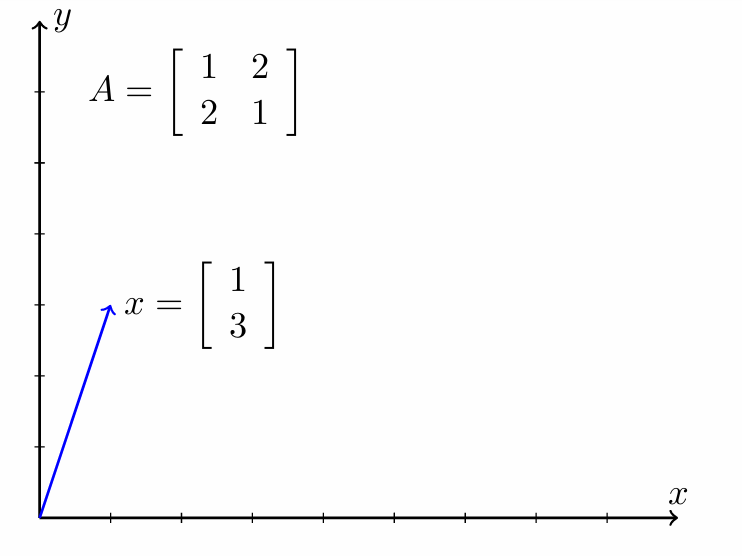
\includegraphics[width=0.9\textwidth]{image_1.png}}
      \only<2->{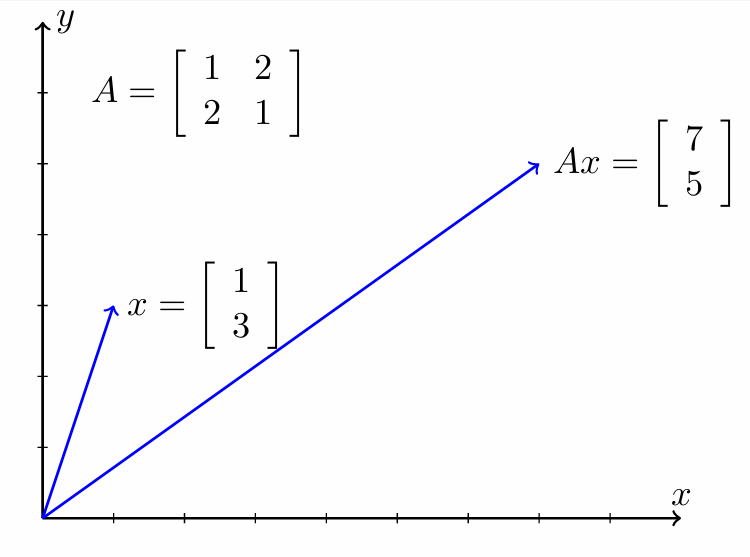
\includegraphics[width=0.9\textwidth]{image_2.png}}
    \end{column}

    % Right Column: Text
    \begin{column}{0.5\textwidth}
      \begin{itemize}
        \item<1-> What happens when a matrix hits a vector?
        
        \item<3-> The vector gets transformed into a new vector (it strays from its path)
        
        \item<3-> The vector may also get scaled (elongated or shortened) in the process.
      \end{itemize}
    \end{column}

  \end{columns}
\end{frame}



\begin{frame}
  \begin{columns}

    % Left Column: Image
    \begin{column}{0.5\textwidth}
      \centering
      \only<1>{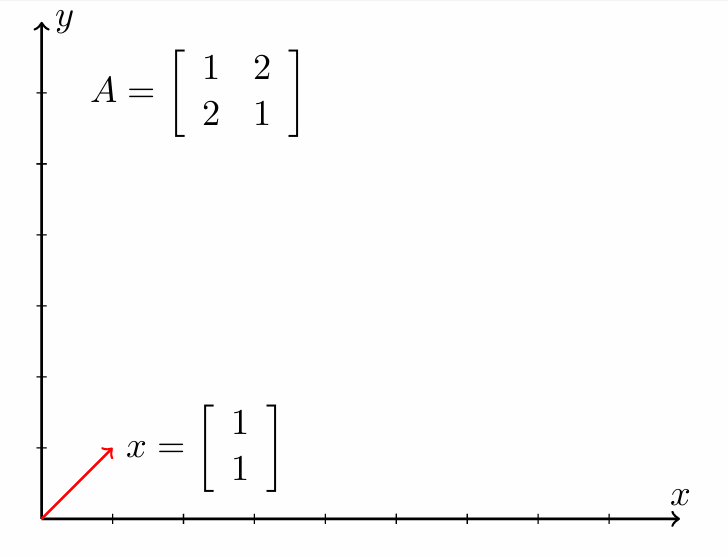
\includegraphics[width=0.9\textwidth]{image_3.png}}
      \only<2->{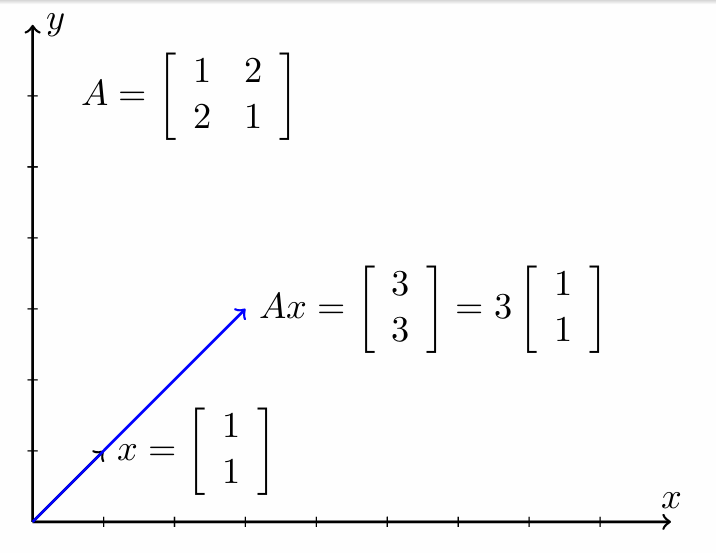
\includegraphics[width=0.9\textwidth]{image_4.png}}
    \end{column}

    % Right Column: Text
    \begin{column}{0.5\textwidth}
      \begin{itemize}
        \item<1-> For a given square matrix A, there exists special vectors which refuse to stray from their path.
        
        \item<3->  These vectors are called \underline{eigenvectors}.
        
        \item<4-> The relative change in magnitude are the corresponding \underline{eigenvalues}.
      \end{itemize}
    \end{column}

  \end{columns}
\end{frame}



\begin{frame}
	\begin{block}{Theorem}
	If $A$ is a square symmetric $n \times n$ matrix, then the solution to the following optimization problem is given by the eigenvector corresponding to the largest eigenvalue of $A$.

\[
\max_{\utilde{x}} \ \utilde{x}^T A \utilde{x} 
\]
\[
\text{s.t. } \|\utilde{x}\| = 1, \ \utilde{x} \in \mathbb{R}^n
\]

and the solution to

\[
\min_{\utilde{x}} \ \utilde{x}^T A \utilde{x} 
\]
\[
\text{s.t. } \|\utilde{x}\| = 1, \ \utilde{x} \in \mathbb{R}^n
\]

is given by the eigenvector corresponding to the smallest eigenvalue of $A$.
	\end{block}

\end{frame}


\begin{frame}
\begin{itemize}
\item<1-> This is a constrained optimization problem that can be solved using Lagrange Multipliers:

\[
L = \utilde{x}^T A \utilde{x} - \lambda (\utilde{x}^T \utilde{x} - 1)
\]

\[
\frac{\partial L}{\partial \utilde{x}} = 2 A \utilde{x} - \lambda (2\utilde{x}) = 0 \Rightarrow A \utilde{x} = \lambda \utilde{x}
\]\\[1em]

\item<2-> Hence $\utilde{x}$ must be an eigenvector of $A$ with eigenvalue $\lambda$. \\[1em]

\item<3-> Multiplying by $\utilde{x}^T$:

\[
\utilde{x}^T A \utilde{x} = \lambda \utilde{x}^T \utilde{x} = \lambda \ (\text{since } \utilde{x}^T \utilde{x} = 1)
\]

\item<4-> Therefore, the critical points of this constrained problem are the eigenvalues of $A$. \\[0.5em]

\item<5-> The maximum value is the largest eigenvalue, while the minimum value is the smallest eigenvalue.
\end{itemize}
\end{frame}

\subsection{Linear Independence and Orthonormal Basis}

\begin{frame}

\begin{block}{Linearly Independent Vectors}
A set of $n$ vectors $v_1, v_2, \ldots , v_n$ is called \textbf{linearly independent} if and only if no vector in the set can be expressed as a linear combination of the remaining $n - 1$ vectors.
\end{block}

\begin{block}{Basis}
A set of vectors $\in \mathbb{R}^n$ is called a \textbf{basis}, if they are linearly independent and every vector $\in \mathbb{R}^n$ can be expressed as a linear combination of these vectors.
\end{block}
\end{frame}


\begin{frame}
  \begin{columns}

    % Left Column: Image
    \begin{column}{0.5\textwidth}
      \centering
      \only<1->{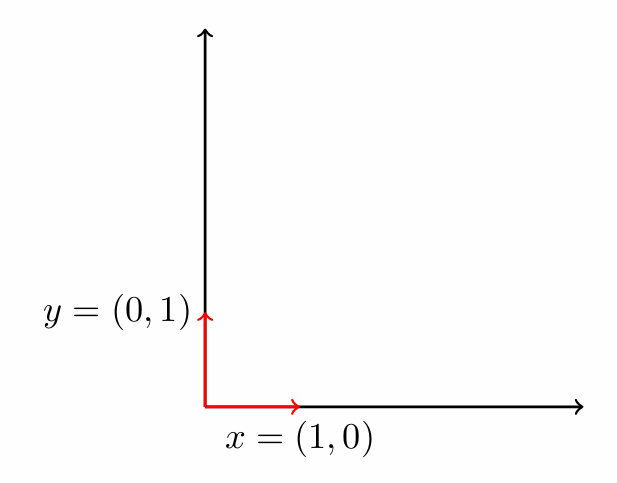
\includegraphics[width=0.9\textwidth]{image_5.png}}
    \end{column}

    % Right Column: Text
    \begin{column}{0.5\textwidth}
      \begin{itemize}
        \item<1-> Consider the space $\mathbb{R}^2$.
        
        \item<2-> Consider two vectors $\utilde{x} =  \begin{bmatrix} 1 \\ 0 \end{bmatrix} $ and $\utilde{y} =  \begin{bmatrix} 0 \\ 1 \end{bmatrix} $.
        
        \item<3-> Any vector $\begin{bmatrix} a \\ b \end{bmatrix}$ can be expressed as a linear combination of these two vectors \textit{i.e.}
        \begin{gather*}
\begin{bmatrix} a \\ b \end{bmatrix}
= 
a \begin{bmatrix} 1 \\ 0 \end{bmatrix}
+
b \begin{bmatrix} 0 \\ 1 \end{bmatrix}.
		\end{gather*}
      \end{itemize}
    \end{column}

  \end{columns}
\end{frame}



\begin{frame}
  \begin{columns}

    % Left Column: Image
    \begin{column}{0.5\textwidth}
      \centering
      \only<1->{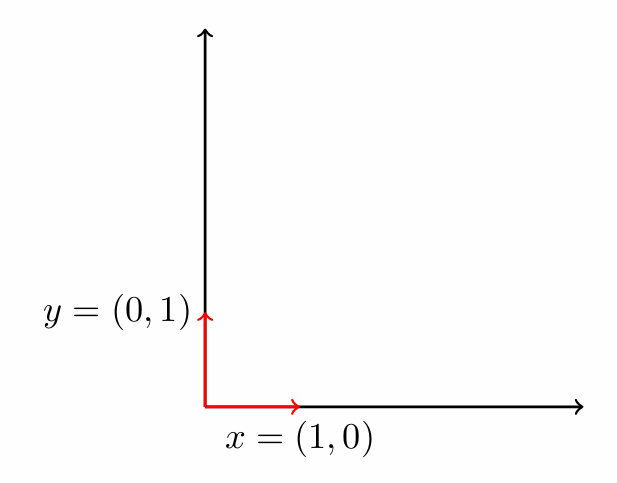
\includegraphics[width=0.9\textwidth]{image_5.png}}
    \end{column}

    % Right Column: Text
    \begin{column}{0.5\textwidth}
      \begin{itemize}
        \item<1-> And indeed we are used to representing all vectors in $\mathbb{R}^2$ as a linear combination of these two vectors.
        
        \item<2-> But there is nothing sacrosanct about this particular choice of $\utilde{x}$ and $\utilde{y}$. 
        
        \item<3-> We could have chosen any 2 linearly independent vectors in $\mathbb{R}^2$ as the basis vectors.    
        \end{itemize}
    \end{column}

  \end{columns}
\end{frame}

\begin{frame}
\begin{itemize}
\item<1-> For example, consider the linearly independent vectors, $\colvec{2}{3}$ and $\colvec{5}{7}$. 

\item<2-> See how any vector $\colvec{a}{b} \in \mathbb{R}^2$ can be expressed as a linear combination of these two vectors.

\begin{gather*}
\colvec{a}{b} = x_1 \colvec{2}{3} + x_2 \colvec{5}{7}.
\end{gather*}

\item<3-> We can find $x_1$ and $x_2$ by solving a system of equations

\begin{align*}
a &= 2x_1 + 5x_2 \\
b &= 3x_1 + 7x_2
\end{align*}

\end{itemize}
\end{frame}


\begin{frame}
  \begin{columns}

    % Left Column: Image
    \begin{column}{0.5\textwidth}
      \centering
      \only<1->{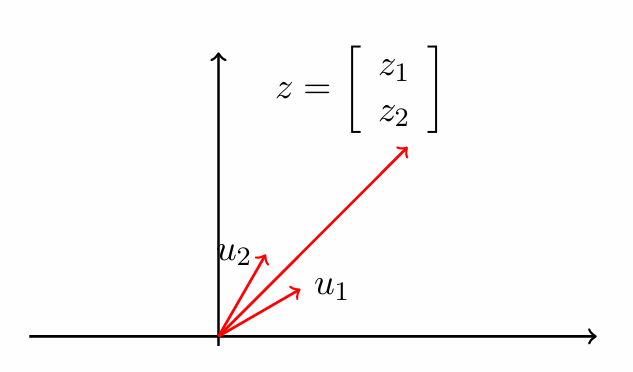
\includegraphics[width=0.9\textwidth]{image_6.png}}
    \end{column}

    % Right Column: Text
    \begin{column}{0.5\textwidth}
      \begin{itemize}
        \item<1-> In general, given a set of linearly independent vectors $$\utilde{u_1}, \utilde{u_2}, \ldots, \utilde{u_n} \in \mathbb{R}^n,$$ we can express any vector $\utilde{z} \in \mathbb{R}^n$ as a linear combination of these vectors. 
        $$ \utilde{z} = \alpha_1 \utilde{u_1} + \alpha_2 \utilde{u_2} + \cdots + \alpha_n \utilde{u_n} $$
        \end{itemize}
    \end{column}

  \end{columns}
\end{frame}

\begin{frame}
\begin{align*}
\utilde{z} &= \alpha_1 \utilde{u_1} + \alpha_2 \utilde{u_2} + \cdots + \alpha_n \utilde{u_n} \\[1.5em]
\Rightarrow \begin{bmatrix}
z_1 \\
z_2 \\
\vdots \\
z_n
\end{bmatrix}
&=
\alpha_1
\begin{bmatrix}
u_{11} \\
u_{12} \\
\vdots \\
u_{1n}
\end{bmatrix}
+
\alpha_2
\begin{bmatrix}
u_{21} \\
u_{22} \\
\vdots \\
u_{2n}
\end{bmatrix}
+ \cdots +
\alpha_n
\begin{bmatrix}
u_{n1} \\
u_{n2} \\
\vdots \\
u_{nn}
\end{bmatrix}
\\[1.5em]
\Rightarrow \begin{bmatrix}
z_1 \\
z_2 \\
\vdots \\
z_n
\end{bmatrix}
&=
\begin{bmatrix}
u_{11} & u_{21} & \cdots & u_{n1} \\
u_{12} & u_{22} & \cdots & u_{n2} \\
\vdots & \vdots & \ddots & \vdots \\
u_{1n} & u_{2n} & \cdots & u_{nn}
\end{bmatrix}
\begin{bmatrix}
\alpha_1 \\
\alpha_2 \\
\vdots \\
\alpha_n
\end{bmatrix}
\end{align*}

We can now find the $\alpha_i$'s using Gaussian Elimination (Time Complexity: $O(N^3))$.
\end{frame}


\begin{frame}
  \begin{columns}

    % Left Column: Image
    \begin{column}{0.5\textwidth}
      \centering
      \only<1->{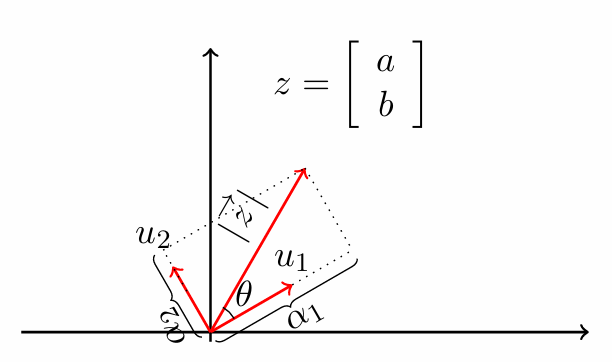
\includegraphics[width=0.9\textwidth]{image_7.png}}
    \end{column}

    % Right Column: Text
    \begin{column}{0.5\textwidth}
      \begin{itemize}
        \item<1-> Now let us see if we have orthonormal basis.
        \item<2-> Then $\utilde{u_i}^T \utilde{u_j} = 0 \ \forall i \neq j$ and $\utilde{u_i}^T \utilde{u_i} = \| \utilde{u_i} \|^2 = 1$.
        \end{itemize}
    \end{column}

  \end{columns}
\end{frame}


\begin{frame}
\begin{itemize}
\item<1-> Now:

\begin{align*}
\utilde{z} &= \alpha_1 \utilde{u_1} + \alpha_2 \utilde{u_2} + \cdots + \alpha_n \utilde{u_n} \\ 
\onslide<2->{\Rightarrow \utilde{u_1}^T \utilde{z} &= \alpha_1 \utilde{u_1}^T \utilde{u_1} + \cdots + \alpha_n \utilde{u_1}^T \utilde{u_n}}\\ \onslide<3->{&= \alpha_1}
\end{align*}

\item<4-> We can directly find each \( \alpha_i \) using a dot product between \( z \) and \( \utilde{u_i} \)
(time complexity \( O(N) \)). \\[0.3cm]

\item<5-> The total complexity will be $O(N^2)$.
\end{itemize}
\end{frame}


\begin{frame}
\begin{block}{Remember}
An orthonormal basis is the most convenient basis that one can hope for.
\end{block}
\end{frame}


\begin{frame}
  \begin{columns}

    % Left Column: Image
    \begin{column}{0.5\textwidth}
      \centering
	  \begin{block}<2->{Theorem}
	  The eigenvectors of a matrix $A \in \mathbb{R}^{n \times n}$ having distinct eigenvalues are linearly independent.
	  \end{block}
	  
	  
	  \begin{block}<3->{Theorem}
	  The eigenvectors of a square symmetric matrix are orthogonal.
	  \end{block}
    \end{column}
      

    % Right Column: Text
    \begin{column}{0.5\textwidth}
      \begin{itemize}
        \item<1-> But what does any of this have to do with eigenvectors?
		\item<2-> Turns out that the eigenvectors can form a basis.
		\item<3-> In fact, the eigenvectors of a square symmetric matrix are even more special.
		\item<4-> Thus they form a very convenient basis.
		\item<5-> Why would we want to use the eigenvectors as a basis instead of the more natural co-ordinate axes?
		\item<6-> We will answer this question soon.
        \end{itemize}
    \end{column}

  \end{columns}
\end{frame}

\subsection{Eigenvalue Decomposition}
\begin{frame}
\begin{itemize}
\item Eigenvalue Decomposition
\end{itemize}
\end{frame}

\begin{frame}
\begin{itemize}
\item<1-> Let $\utilde{u_1}, \utilde{u_2}, \ldots, \utilde{u_n}$ be the eigenvectors of a square matrix $A$ and let $\lambda_1, \lambda_2, \ldots, \lambda_n$ be the corresponding eigenvalues. \\[0.5em]

\item<2-> Consider a matrix $U$ whose columns are $\utilde{u_1}, \utilde{u_2}, \ldots, \utilde{u_n}$. \\[0.5em]

\item<3-> Now

\begin{align*}
AU \onslide<3->{&= A \begin{bmatrix}
\uparrow & \uparrow & & \uparrow \\
\utilde{u_1} & \utilde{u_2} & \cdots & \utilde{u_n} \\
\downarrow & \downarrow & & \downarrow
\end{bmatrix}}
\onslide<4->{= \begin{bmatrix}
\uparrow & \uparrow & & \uparrow \\
A\utilde{u_1} & A\utilde{u_2} & \cdots & A\utilde{u_n} \\
\downarrow & \downarrow & & \downarrow
\end{bmatrix}}
\onslide<5->{= \begin{bmatrix}
\uparrow & \uparrow & & \uparrow \\
\lambda_1 \utilde{u_1} & \lambda_2 \utilde{u_2} & \cdots & \lambda_n \utilde{u_n} \\
\downarrow & \downarrow & & \downarrow
\end{bmatrix}} \\
\onslide<6->{&= \begin{bmatrix}
\uparrow & \uparrow & & \uparrow \\
\utilde{u_1} & \utilde{u_2} & \cdots & \utilde{u_n} \\
\downarrow & \downarrow & & \downarrow
\end{bmatrix} \cdot
\begin{bmatrix}
\lambda_1 & 0 & \cdots & 0 \\
0 & \lambda_2 & \cdots & \vdots \\
\vdots & \vdots & \ddots & 0 \\
0 & \cdots & 0 & \lambda_n
\end{bmatrix}}
\onslide<7->{= U \Lambda}
\end{align*}

\onslide<8->{where $\Lambda$ is a diagonal matrix whose diagonal elements are the eigenvalues of $A$.}
\end{itemize}
\end{frame}

\begin{frame}
\onslide<1->{$$\therefore \,\,  AU = U\Lambda$$.}

\onslide<2->{Now, if the columns of $U$ are linearly independent} \\ \onslide<3->{\textit{i.e.} if $A$ has $n$ linearly independent eigenvectors} \\
\onslide<4->{\textit{i.e.} if $A$ has $n$ distinct eigenvalues,} \\[1em] \onslide<5->{then $U^{-1}$ exists and we can write}

\begin{align*}
\onslide<6->{A &= U \Lambda U^{-1} \hspace{0.2cm} \text{[eigenvalue decomposition]}} \\
\onslide<7->{U^{-1} A U &= \Lambda \hspace{1.2cm} \text{[diagonalization of } A]}
\end{align*}
\end{frame}


\begin{frame}
\begin{itemize}
\item<1-> If $A$ is symmetric then the situation is even more convenient. 
\item<2-> The eigenvectors are orthogonal. 
\item<3-> Further let's assume, that the eigenvectors have been normalized. $$\left[ \utilde{u_i}^T \utilde{u_i} = 1 \right]$$

\item<4-> Then,
\[
Q = U^T U =
\onslide<5->{\begin{bmatrix}
\leftarrow u_1 \rightarrow \\
\leftarrow u_2 \rightarrow \\
\vdots \\
\leftarrow u_n \rightarrow
\end{bmatrix}}
\onslide<6->{\begin{bmatrix}
\uparrow & \uparrow & & \uparrow \\
u_1 & u_2 & \cdots & u_n \\
\downarrow & \downarrow & & \downarrow
\end{bmatrix}}
\]

\onslide<7->{Each entry of the matrix, $Q_{ij}$ is given by $\utilde{u_i}^T \utilde{u_j}$}

\[
\onslide<8->{
Q_{ij} = \utilde{u_i}^T \utilde{u_j} =
\begin{cases}
0 & \text{if } i \neq j \\
1 & \text{if } i = j
\end{cases}} \,\,
\onslide<9->{\therefore \,\, U^T U = \mathbb{I} \ \text{(the identity matrix)}}
\]

\onslide<10->{So $U^T$ is the inverse of $U$ (very convenient to calculate).}
\end{itemize}
\end{frame}

\begin{frame}
\begin{block}{The story so far \ldots}

\begin{itemize}

\item<1-> The eigenvectors corresponding to different eigenvalues are linearly independent.

\item<2-> The eigenvectors of a square symmetric matrix are orthogonal.

\item<3-> The eigenvectors of a square symmetric matrix can thus form a convenient basis.

\end{itemize}

\end{block}

\onslide<4->{We will put all these to use.}
\end{frame}


\section{Principal Component Analysis}

\subsection{Interpretation 1}
\begin{frame}{Principal Component Analysis}
\begin{itemize}
\item Interpretation 1
\end{itemize}
\end{frame}



\begin{frame}
  \begin{columns}

    % Left Column: Image
    \begin{column}{0.5\textwidth}
      \centering
      \only<1->{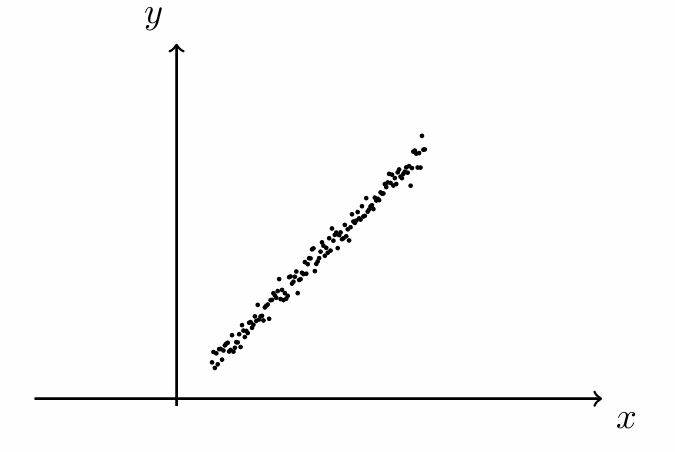
\includegraphics[width=0.9\textwidth]{image_8.png}}	  
    \end{column}
      

    % Right Column: Text
    \begin{column}{0.5\textwidth}
      \begin{itemize}
        \item<1-> Consider the following data.
		\item<2-> Each point (vector) here is represented using a linear combination of the $x$ and $y$ axes (\textit{i.e.} using the point’s $x$ and $y$ co-ordinates).
		\item<3-> In other words we are using $x-$axis and $y-$axis as the basis.
		\item<4-> What if we choose a different basis?
        \end{itemize}
    \end{column}

  \end{columns}
\end{frame}



\begin{frame}
  \begin{columns}

    % Left Column: Image
    \begin{column}{0.5\textwidth}
      \centering
      \only<1->{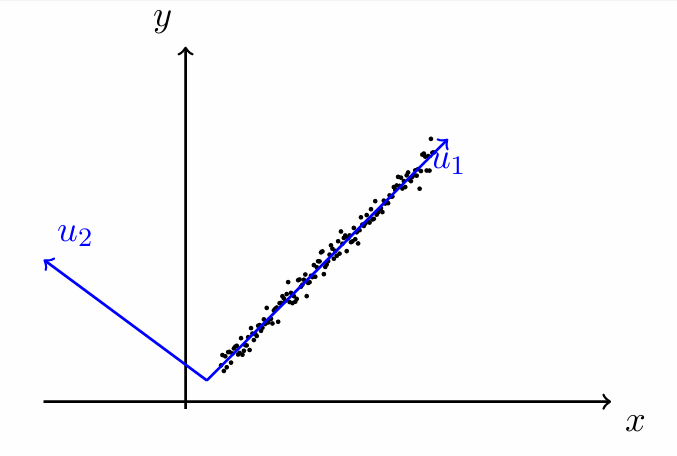
\includegraphics[width=0.9\textwidth]{image_9.png}}	  
    \end{column}
      

    % Right Column: Text
    \begin{column}{0.5\textwidth}
      \begin{itemize}
        \item<1-> For example, what if we use $\utilde{u_1}$ and $\utilde{u_2}$ as a basis instead of $x-$axis and $y-$axis.
		\item<2-> We observe that all the points have a
very small component in the direction of $\utilde{u_2}$ (almost noise).
		\item<3-> It seems that the same data which was originally in $\mathbb{R}^2 (x, y)$ can now be represented in $\mathbb{R}^1(u_1)$ by making a smarter choice for the basis.
        \end{itemize}
    \end{column}

  \end{columns}
\end{frame}


\begin{frame}
  \begin{columns}

    % Left Column: Image
    \begin{column}{0.5\textwidth}
      \centering
      \only<1-2>{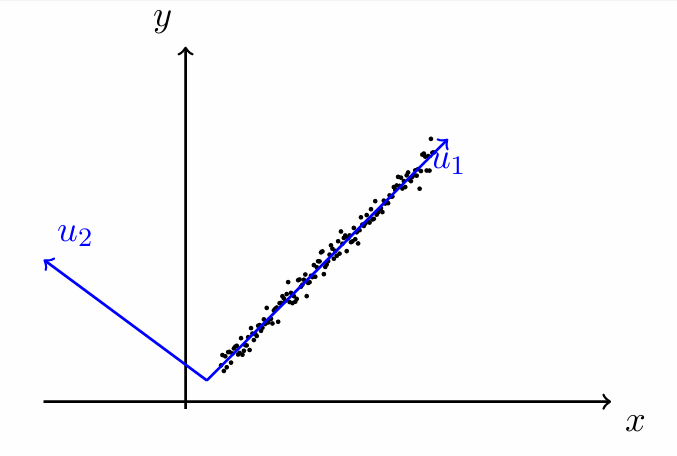
\includegraphics[width=0.9\textwidth]{image_9.png}}
	  \only<3->{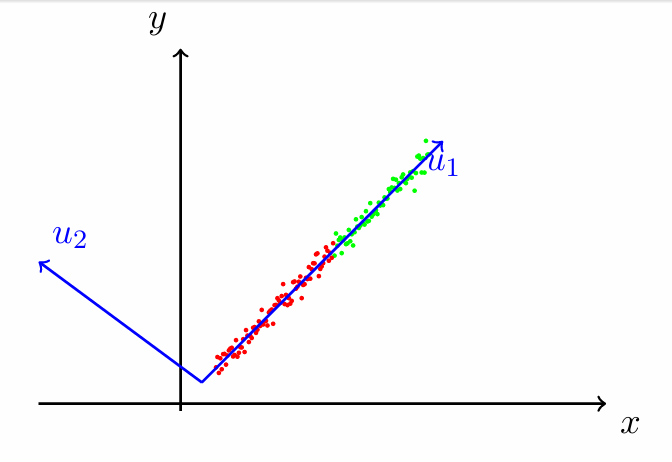
\includegraphics[width=0.9\textwidth]{image_10.png}}
    \end{column}
      

    % Right Column: Text
    \begin{column}{0.5\textwidth}
      \begin{itemize}
        \item<1-> But why not care about $\utilde{u_2}$ ?
		\item<2-> Because the variance in the data in this direction is very small (all data points have almost the same value in the $\utilde{u_2}$ direction).
		\item<3-> If we were to build a classifier on top of this data then $\utilde{u_2}$ would not contribute to the classifier as the points are not distinguishable along this direction.
        \end{itemize}
    \end{column}

  \end{columns}
\end{frame}


\begin{frame}
\begin{block}{Remember}
In general, we are interested in representing the data using \underline{fewer dimensions} such that the data has \underline{high variance} along these dimensions. 
\end{block}

But that's not all.
\end{frame}

\begin{frame}
\begin{columns}

    % Left Column: Image
    \begin{column}{0.5\textwidth}
      \centering
      \only<1->{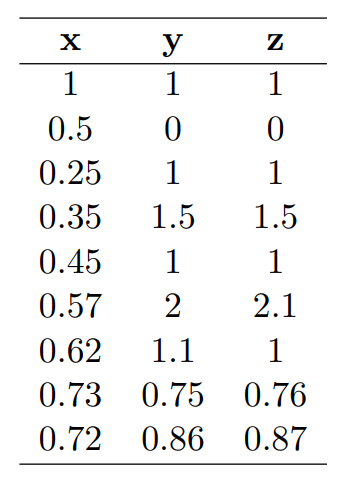
\includegraphics[scale=0.5]{image_11.png}}
    \end{column}
      

    % Right Column: Text
    \begin{column}{0.5\textwidth}
      \begin{itemize}
        \item<1-> Consider the following data.
		\item<2-> Notice that $y$ and $z$ are highly correlated.
		\item<3-> So $z$ adds no new information beyond what is already contained in $y$.
		\item<4-> In other words, $z$ is redundant as it is largely linearly dependent on $y$.
        \end{itemize}
    \end{column}

  \end{columns}
\end{frame}

\begin{frame}
\begin{block}{\scalebox{1.5}{\twemoji{bullseye}} Remember}
\onslide<1->{So in general, in PCA, we are interested in representing the data using \underline{fewer dimensions}} \\
\onslide<2->{chopping off dimensions  \scalebox{1.5}{\twemoji{cross mark}}, transforming the data \scalebox{1.5}{\twemoji{check mark button}}} \\ \onslide<3->{such that}

\begin{itemize}

\item<4-> The data has \underline{high variance} along these dimensions;

\item<5-> The dimensions are \underline{linearly independent} (uncorrelated); even better if they are orthogonal because that will be a very convenient basis. \\

\end{itemize}

\end{block}
\end{frame}

\begin{frame}
\begin{itemize}
\item<1-> Now let $\utilde{p_1}, \utilde{p_2}, \ldots , \utilde{p_n}$ be a set of such $n$ linearly independent orthonormal vectors. Let $P$ be a $n \times n$ matrix such that $\utilde{p_1}, \utilde{p_2}, \ldots , \utilde{p_n}$ are the columns of $P$. \\

\item<2-> Let $\utilde{x_1}, \utilde{x_2}, \ldots , \utilde{x_m} \in \mathbb{R}^n$ be $m$ data points and let $X$ be a matrix such that $\utilde{x_1}, \utilde{x_2}, \ldots , \utilde{x_m}$ are the rows of this matrix. Further let us assume that the data is $0-$mean and unit variance. \\

\item<3-> We want to represent each $\utilde{x_i}$ using this new basis $P$ as follows.

$$\utilde{x_i} = \alpha_{i1} \utilde{p_1} + \alpha_{i2} \utilde{p_2} + \alpha_{i3} \utilde{p_3} + \ldots + \alpha_{in} \utilde{p_n}.$$

\item<4-> For an orthonormal basis we know that we can find these $\alpha_{ij}'$s using

\[
\alpha_{ij} = \utilde{x_i}^T \utilde{p_j} = 
\left[
\leftarrow \; \utilde{x_i} \; \rightarrow
\right]
\begin{bmatrix}
\uparrow \\
\utilde{p_j} \\
\downarrow
\end{bmatrix}
\]
\end{itemize}
\end{frame}

\begin{frame}
\begin{itemize}
\item<1-> In general, the transformed data $\utilde{\hat{x}_i}$ is given by

\[
\onslide<2->{\utilde{\hat{x}_i} = 
\left[ \leftarrow \; \utilde{x_i} \; \rightarrow \right]
\begin{bmatrix}
\uparrow & & \uparrow \\
\utilde{p_1} & \cdots & \utilde{p_n} \\
\downarrow & & \downarrow
\end{bmatrix}}
\onslide<3->{= \utilde{x_i}^T P} 
\onslide<4->{= \left( \alpha_{i1}, \alpha_{i2}, \ldots, \alpha_{in} \right)_{1 \times n}}
\]

\onslide<5->{
and

 \[
\hat{X} = X P
\qquad (\hat{X} \text{ is the matrix of transformed points})
\]}
\end{itemize}
\end{frame}


\begin{frame}
\begin{block}<1->{Theorem}
If $X$ is a matrix such that its columns have zero mean and if $\hat{X} = X P$ then the columns of $\hat{X}$ will also have zero mean.

\textbf{Proof :} For any matrix $A$, $\mathbf{1}^T A$ gives us a row vector with the $i^{th}$ element containing the sum of the $i^{th}$ column of $A$. (This is easy to see using the row-column picture of matrix multiplication). \\
Consider
\[
\mathbf{1}^T \hat{X} = \mathbf{1}^T X P = \left(\mathbf{1}^T X\right) P
\]
But $\mathbf{1}^T X$ is the row vector containing the sums of the columns of $X$. Thus $\mathbf{1}^T X = \utilde{0}$. Therefore, $\mathbf{1}^T \hat{X} = \utilde{0}$. \\
Hence the transformed matrix also has columns with sum = 0.
\end{block}

\begin{block}<2->{Theorem}
$X^T X$ is a symmetric matrix. \\
\textbf{Proof :} We can write
$ \left( X^T X \right)^T = X^T \left( X^T \right)^T = X^T X $.
\end{block}
\end{frame}

\begin{frame}
\begin{block}{Result}
If $X$ is a matrix whose columns are zero mean then $\Sigma = \dfrac{1}{m} X^T X$ is the covariance matrix. In other words, each entry $\sigma_{ij}$ stores the covariance between columns $i$ and $j$ of $X$.

\onslide<1->{\textbf{Explanation} : Let $\Sigma$ be the covariance matrix of $X$. Let $\mu_i, \mu_j$ denote the means of the $i^{th}$ and $j^{th}$ column of $X$ respectively.} \onslide<2->{Then by definition of covariance, we can write:}

\begin{align*}
\onslide<3->{\sigma_{ij} &= \dfrac{1}{m} \sum\limits_{k=1}^{m} (X_{ki} - \mu_i)(X_{kj} - \mu_j)} \\
\onslide<4->{&= \dfrac{1}{m} \sum\limits_{k=1}^{m} X_{ki} X_{kj} \hspace{1cm} [\because \mu_i = \mu_j = 0]} \\
\onslide<5->{&= \dfrac{1}{m} X_i^T X_j}
\onslide<6->{= \left( \dfrac{1}{m}  X^T X \right)_{ij}}
\end{align*}
\end{block}
\end{frame}

\begin{frame}
\begin{itemize}
\item<1-> We have $\hat{X} = X P$. 
\item<2-> Using the previous theorems \& result, we get $\dfrac{1}{m} \hat{X}^T \hat{X}$ is the covariance matrix of the transformed data. We can write:
    \[
    \onslide<3->{\dfrac{1}{m} \hat{X}^T \hat{X}} \onslide<4->{= \dfrac{1}{m} (X P)^T X P} \onslide<5->{= \dfrac{1}{m} P^T X^T X P} \onslide<6->{= P^T \left(\dfrac{1}{m} X^T X\right) P} \onslide<7->{= P^T \Sigma P}
    \]
    
\item<8-> We know each cell $i, j$ of the covariance matrix $\dfrac{1}{m} \hat{X}^T \hat{X}$ stores the covariance between columns $i$ and $j$ of $\hat{X}$. 

\item<9-> Ideally, we want
\begin{align*}
\onslide<10->{\left(\dfrac{1}{m} \hat{X}^T \hat{X}\right)_{ij} &= 0 \qquad \text{if } i \neq j \ (\text{covariance = 0})} \\
\onslide<11->{\left(\dfrac{1}{m} \hat{X}^T \hat{X}\right)_{ij} &\neq 0 \qquad \text{if } i = j \ (\text{variance } \neq 0)}
\end{align*}
    
\item<12-> In other words, we want
\[
\onslide<13->{\dfrac{1}{m} \hat{X}^T \hat{X} = P^T \Sigma P} \onslide<14->{= D. \hspace{1cm} \text{[ where D is a diagonal matrix ]}}
\]
\end{itemize}
\end{frame}


\begin{frame}
\begin{itemize}
\item<1-> We want $P^T \Sigma P = D$ where $\Sigma$ is a square matrix and $P$ is an orthogonal matrix.

\item<2-> Now the question is which orthogonal matrix satisfies the following condition $P^T \Sigma P = D $ .

\item<3-> In other words, which orthogonal matrix $P$ diagonalizes $\Sigma$? 

\item<4-> Answer is a matrix $P$ whose columns are the eigenvectors of $\Sigma = \dfrac{1}{m} X^T X$ [by Eigenvalue Decomposition]. \\

\item<5-> Thus, the new basis $P$ used to transform $X$ is the basis consisting of the eigenvectors of $\dfrac{1}{m} X^T X$. \\
\end{itemize}
\end{frame}

\begin{frame}
\begin{itemize}
\item<1-> Why is this a good basis? 
\item<2-> Because the eigenvectors of $\dfrac{1}{m}X^T X$ are linearly independent and because the eigenvectors of $\dfrac{1}{m}X^T X$ are orthogonal.

\item<3-> This method is called Principal Component Analysis for transforming the data to a new basis where the dimensions are non-redundant (low covariance) \& not noisy (high variance).

\item<4-> In practice, we select only the top-$k$ dimensions along which the variance is high (this will become more clear when we look at an alternate interpretation of PCA).
\end{itemize}
\end{frame}


\subsection{Interpretation 2}
\begin{frame}{Principal Component Analysis}
\begin{itemize}
\item Interpretation 2
\end{itemize}
\end{frame}

\begin{frame}
\onslide<1->{Given $n$ orthonormal linearly independent vectors $\utilde{p_1}, \utilde{p_2}, \ldots, \utilde{p_n}$,} \onslide<2->{we can represent $\utilde{x_i}$ \underline{exactly} as a linear combination of these vectors as follows.
\[
\utilde{x_i} = \sum_{j=1}^{n} \alpha_{ij} \utilde{p_j} \hspace{0.5cm}  \text{[we know how to estimate $\alpha_{ij}$'s but we will come back to that later]}
\]}

\onslide<3->{But we are interested only in the top-$k$ dimensions (we want to get rid of noisy \& redundant dimensions)
\[
\utilde{\hat{x}_i} = \sum_{j=1}^{k} \alpha_{ij} \utilde{p_j}
\]}

\onslide<4->{So we want to select $p_i$'s such that we minimise the \underline{reconstruction error} :
\[
e = \sum_{i=1}^{m} (\utilde{x_i} - \utilde{\hat{x}_i})^T (\utilde{x_i} - \utilde{\hat{x}_i})
\]}
\end{frame}


\begin{frame}
Now, 
\begin{align*}
\onslide<1->{e &= \sum_{i=1}^{m} (\utilde{x_i} - \utilde{\hat{x}_i})^T (\utilde{x_i} - \utilde{\hat{x}_i})} \\[0.75em]
\onslide<2->{&= \sum_{i=1}^m \left( \sum_{j=1}^n \alpha_{ij} \utilde{p_j} - \sum_{j=1}^k \alpha_{ij} \utilde{p_j} \right)^T \left( \sum_{j=1}^n \alpha_{ij} \utilde{p_j} - \sum_{j=1}^k \alpha_{ij} \utilde{p_j} \right)} \\[0.75em]
\onslide<3->{&= \sum_{i=1}^m \left[ \left( \sum_{j=k+1}^n \alpha_{ij} p_j \right)^T \left( \sum_{j=k+1}^n \alpha_{ij} p_j \right) \right]} \\[0.75em]
\onslide<4->{&= \sum_{i=1}^m \left( \alpha_{i,k+1} \cdot \utilde{p_{k+1}} + \alpha_{i,k+2} \cdot \utilde{p_{k+2}} + \ldots + \alpha_{i,n} \cdot \utilde{p_n} \right)^T \cdot \\
&\hspace{2cm}\left( \alpha_{i,k+1} \cdot \utilde{p_{k+1}} + \alpha_{i,k+2} \cdot \utilde{p_{k+2}} + \ldots + \alpha_{i,n} \cdot \utilde{p_n} \right)}
\end{align*}
\end{frame}

\begin{frame}
\begin{align*}
\onslide<1->{&= \sum_{i=1}^m \left( \alpha_{i,k+1} \cdot \utilde{p_{k+1}}^T + \alpha_{i,k+2} \cdot \utilde{p_{k+2}}^T + \ldots + \alpha_{i,n} \cdot \utilde{p_n}^T \right) \cdot \\
&\hspace{2cm} \left( \alpha_{i,k+1} \cdot \utilde{p_{k+1}} + \alpha_{i,k+2} \cdot \utilde{p_{k+2}} + \ldots + \alpha_{i,n} \cdot \utilde{p_n} \right)} \\[0.75em]
\onslide<2->{&= \sum_{i=1}^m \left( \sum_{j=k+1}^n \alpha_{ij} \utilde{p_j}^T \cdot \alpha_{ij} \utilde{p_j} \right)} \onslide<3->{+ \sum_{i=1}^m \left( \sum_{j=k+1}^n \sum_{L=k+1, L \neq k}^n \alpha_{ij} \utilde{p_j}^T \cdot \alpha_{iL} \utilde{p_L} \right)} \\[0.75em]
\onslide<4->{&= \sum_{i=1}^m \sum_{j=k+1}^n \alpha_{ij} \utilde{p_j}^T \utilde{p_j} \alpha_{ij} + \sum_{i=1}^m \sum_{j=k+1}^n \sum_{L=k+1, L \neq k}^n \alpha_{ij} \utilde{p_j}^T \utilde{p_L} \alpha_{iL}} \\[0.75em]
\onslide<5->{&= \sum_{i=1}^m \sum_{j=k+1}^n \alpha_{ij}^2 \qquad 
(\because \utilde{p_j}^T \utilde{p_j} = 1, \ \utilde{p_i}^T \utilde{p_j} = 0 \,\, \forall i \neq j)}
\end{align*}
\end{frame}


\begin{frame}
\begin{align*}
\onslide<1->{&= \sum_{i=1}^m \sum_{j=k+1}^n \left( \utilde{x_i}^T \utilde{p_j} \right)^2} \\[0.75em] 
\onslide<2->{&= \sum_{i=1}^{m} \sum_{j=k+1}^{n} \left( \utilde{p_j}^T x_i \right) \left( x_i^T \utilde{p_j} \right)} \\[0.75em]
\onslide<3->{&= \sum_{j=k+1}^{n} \utilde{p_j}^T \left( \sum_{i=1}^{m} \utilde{x_i} \utilde{x_i}^T \right) \utilde{p_j}} \\[0.75em]
\onslide<4->{&= \sum_{j=k+1}^{n} \utilde{p_j}^T \, m \Sigma \, \utilde{p_j} \qquad \left[ \because \frac{1}{m} \sum_{i=1}^{m} \utilde{x_i} \utilde{x_i}^T = \frac{X^T X}{m} = \Sigma \right]}
\end{align*}
\end{frame}


\begin{frame}
\begin{itemize}
\item<1-> So we want to minimize
\[
\min_{\utilde{p_{k+1}}, \utilde{p_{k+2}}, \ldots, \utilde{p_n}} \sum_{j=k+1}^{n} \utilde{p_j}^T m \Sigma \utilde{p_j}
\qquad \text{s.t. } \utilde{p_j}^T \utilde{p_j} = 1 \quad \forall j = k+1, k+2, \ldots, n
\]

\item<2-> The solution to the above problem is given by the eigenvectors corresponding to the smallest eigenvalues of $\Sigma$.

\item<3-> Thus we select $\utilde{p_1}, \utilde{p_2}, \ldots, \utilde{p_n}$ as eigenvectors of $\Sigma$ and retain only top-$k$ eigenvectors to express the data [or discard the eigenvectors $\utilde{p_{k+1}}, \utilde{p_{k+2}}, \ldots, \utilde{p_n}$].

\item<4-> Here the key idea was to minimize the error in reconstructing $\utilde{x_i}$ after projecting the data on to a new basis.
\end{itemize}
\end{frame}

\begin{frame}
\begin{block}{$\spadesuit$ A quick recap}
\begin{itemize}
\item<1-> The eigenvectors of a matrix with distinct eigenvalues are linearly independent.
\item<2-> The eigenvectors of a square symmetric matrix are orthogonal.
\item<3-> PCA exploits this fact by representing the data using a new basis comprising only the top-$k$ eigenvectors.
\item<4-> The $n - k$ dimensions which contribute very little to the reconstruction error are discarded. These are also the directions along which the variance is minimum (we shall establish this in yet another interpretation of PCA).
\end{itemize}
\end{block}
\end{frame}

\subsection{Interpretation 3}
\begin{frame}{Principal Component Analysis}
\begin{itemize}
\item Interpretation 3
\end{itemize}
\end{frame}


\begin{frame}
\begin{itemize}
\item<1-> We started off with the following wishlist. \\

\begin{itemize}
\item<2-> the dimensions have low covariance
\item<3-> the dimensions have high variance
\end{itemize}

\item<4-> So far we have paid a lot of attention to the covariance. But what about variance? Have we achieved our stated goal of high variance along dimensions? 

\item<5-> To answer this question we will see yet another interpretation of PCA.
\end{itemize}
\end{frame}

\begin{frame}
\begin{itemize}
\item<1-> The \( i^{\text{th}} \) dimension of the transformed data \( \hat{X} \) is given by $\utilde{\hat{X}_i} = Xp_i$.

\item<2-> The variance along this dimension is given by
\begin{align*}
\onslide<3->{\dfrac{\utilde{\hat{X}_i}^T \utilde{\hat{X}_i}}{m} &= \dfrac{1}{m} \utilde{p_i}^T X^T X \utilde{p_i}} \\
\onslide<4->{&= \utilde{p_i}^T \underbrace{\dfrac{1}{m} X^T X \utilde{p_i}}} \\
\onslide<5->{&= \utilde{p_i}^T \underbrace{\Sigma \utilde{p_i}} \\
&= \utilde{p_i}^T \lambda_i \utilde{p_i} \qquad [\because \utilde{p_i} \text{ is an eigenvector of } \Sigma]}  \\
\onslide<6->{&= \lambda_i \underbrace{\utilde{p_i}^T \utilde{p_i}}_{=1}} \\
\onslide<7->{&= \lambda_i}
\end{align*}
\end{itemize}
\end{frame}

\begin{frame}
\begin{itemize}
\item<1-> Thus the variance along the \( i^{\text{th}} \) dimension (\( i^{\text{th}} \) eigenvector of \( \Sigma \)) is given by the corresponding eigenvalue.
\item<2-> Hence, we did the right thing by discarding the dimensions (eigenvectors) corresponding to lower eigenvalues!
\end{itemize}
\end{frame}


\begin{frame}
\begin{block}{$\spadesuit$ A Quick Summary}
We have seen 3 different interpretations of PCA.
\begin{itemize}
\item<1-> It ensures that the covariance between the new dimensions are minimized.
\item<2-> It picks up dimensions such that the data exhibit high variance across these dimensions.
\item<3-> It ensures that the data can be represented using less number of dimensions.
\end{itemize}
\end{block}
\end{frame}


\begin{frame}
\begin{block}{$\spadesuit$ Total Variance}
The total variability caused by the initial feature set \textit{i.e.} $\utilde{X_1}, \utilde{X_2}, \ldots, \utilde{X_n}$ is same as the total variability caused by the transformed feature set \textit{i.e.} $\utilde{\hat{X_1}}, \utilde{\hat{X_2}}, \ldots, \utilde{\hat{X_n}}$. How ? 
\begin{align*}
\onslide<1->{\text{Total variation due to } \utilde{X_1}, \utilde{X_2}, \ldots, \utilde{X_n} &= \text{sum of the principal diagonal elements of } \Sigma} \\[0.75em]
\onslide<2->{&= \text{trace }(\Sigma)} \\[0.75em]
\onslide<3->{&= \text{sum of the eigenvalues of }\Sigma} \\[0.75em]
\onslide<4->{&= \text{Total variation due to } \utilde{\hat{X_1}}, \utilde{\hat{X_2}}, \ldots, \utilde{\hat{X_n}}.}
\end{align*}
\end{block}
\end{frame}

\end{document}